\chapter{Computational Methodology}

\label{ch:compmethodology}

\section{Density functional theory} \label{section:dft}

Quantum mechanics is currently the most complete modern theory which describes the behaviour of matter at the length scale of atoms. It can be used to predict things such as the energy levels of atoms, the interactions of light with matter, and the thermodynamic stability of systems of atoms. Ideally, the mathematical formalisms of quantum mechanics would be used to predict the properties and behaviour of all possible types of molecules and materials. In reality, this is very difficult to achieve, requiring several approximations and abstractions in order to produce methods which, sacrifice some degree of physical accuracy in order to be computationally tractable. Currently, the most successful approach to predict the behaviour of most solids is provided by density functional theory.
% The mathematical formalisms of quantum mechanics must themselves be discretised to be used in computational simulation methods.

\subsection{The Schr\"{o}dinger equation}

The time-independent Schr\"{o}dinger equation is used to find the total energy of a system:
\begin{equation}
E\Psi(\textbf{r}) = \hat{H}\Psi(\textbf{r})
\label{equation:schrodinger}
\end{equation}

where $E$ is the total energy of the system, $\Psi$ is the wave function associated with the electrons, and $\hat{H}$ is the energy Hamiltonian operator. $\hat{H}$ includes the kinetic energy contributions ($\hat{T}$) and potential energy contributions ($\hat{V}$), shown in atomic units in equations \ref{equation:kineticcontribution} and \ref{equation:potentialcontribution} respectively:
\begin{gather}
\hat{H} = \hat{T} + \hat{V} \label{equation:hamiltonian}\\
\hat{T} = -\sum_i{\frac{1}{2}}\nabla^2_{r_i} - \sum_i{\frac{1}{2M_i}}\nabla^2_{R_i} \label{equation:kineticcontribution} \\
\hat{V} = \sum_{i,j=i+1}{\frac{1}{2|r_i - r_j|}} + \sum_{i,j=i+1}{\frac{Z_i Z_j}{2|R_i - R_j|}} - \sum_{i,j}{\frac{Z_i}{2|R_i - r_j|}} \label{equation:potentialcontribution}
\end{gather}

where $r_{i}$ is the position of electron $i$, $R_{i}$ is the position of nucleus $i$ and $M_{i}$ is the mass of nucleus $i$. Thus, the second term on the right of equation \ref{equation:kineticcontribution} relates to the kinetic energy of any associated nuclei, and the first term to electrons. 

If $\Psi(\textbf{r})$ is the wave function, the electron density at position \textbf{r} ($\rho(\textbf{r})$) is given by:
\begin{equation}
\rho(\textbf{r}) = \Psi(\textbf{r})^2
\end{equation}

\subsection{Kohn-Sham Method} \label{section:kohnsham}

Density Functional Theory (DFT) was developed by Kohn and Sham in 1964 \cite{Kohn1965} as an ab initio method for predicting $\rho(\textbf{r})$ associated with an ensemble of atoms. The Kohn-Sham Hamiltonian (Equation \ref{equation:kohnsham}) is used in the Schr\"odinger equation.
\begin{equation}
\hat{H}(\rho(\textbf{r})) = E_{KE}(\rho(\textbf{r})) + E_{P}(\rho(\textbf{r})) + E_{XC}(\rho(\textbf{r}))
\label{equation:kohnsham}
\end{equation}

Where $E_{KE}$ and $E_{P}$ are the kinetic and potential energy functionals (functions of functions), $E_{XC}$ is the exchange correlation functional, and \textbf{r} is the position vector. The main approximation is to consider that the electrons only interact with nuclei and the average field generated by all other electrons, and not other electrons explicitly, thus allowing all the terms to be evaluated using the electron density rather than position. An exchange correlation term is then used to include the non-classical electron-electron interactions, namely electron exchange and correlation. Additionally, the exchange correlation term includes the difference in kinetic energy due to the use of non-interacting electrons. While Kohn and Sham did provide a proof for the existence of an exchange correlation function, a general form of the functional has not yet been found, although several forms have been considered, each with strengths and weaknesses when applied to different systems. One basic form of the functional which is frequently used is the local density approximation (LDA) \cite{Kohn1965}:
\begin{equation}
E_{LDA}(\rho(\textbf{r})) = \int\rho(\textbf{r})e_{uniform}(\rho(\textbf{r}))dr
\label{equation:LDA}
\end{equation}

where $e_{uniform}$ is the normalised exchange-correlation energy of a uniform electron gas (an idealised system). This exchange-correlation functional generates accurate results in materials such as metals where the electron density is relatively uniform, while systems with more rapidly changing electron densities (e.g. highly ionic materials) require more complex functionals. A natural extension of the LDA is to also take into account the gradient of the electron density, thus allowing a smoother functional fit when electron density is highly variable as a function of position. Such functionals are collectively referred to as generalised gradient approximations (GGAs) \cite{Langreth1980, Langreth1983, Becke1988, perdew2008restoring}. One GGA which has enjoyed widespread use for many different types of systems is the Perdew-Burke-Ernzerhof (PBE) GGA \cite{Perdew1996}. The accuracy of this functional when modelling solid phase systems is well-established, and its frequent use in DFT studies provides ample reference material for comparing results. After conducting several convergence tests (see § \ref{section:convergence}), the PBE GGA was chosen as the exchange-correlation functional to be used for all calculations in this thesis.

\subsubsection{Born-Oppenheimer approximation}

The Born-Oppenheimer approximation is a two-step process for evaluating atomic forces, which greatly reduces the computational costs of any atomistic simulation. It exploits the large difference in mass between nuclei and electrons in order to separate their interactions. This allows us to decompose the total wave function into a product of an electronic wave function and a nuclear wave function via a separation of variables approach. The first step involves ignoring the kinetic energy contribution of nuclei by assuming they are stationary, thus the nuclear kinetic energy term in Equation \ref{equation:kineticcontribution} can be removed. The stationary nuclei assumption also simplifies the nuclear-nuclear Coulombic repulsion term in Equation \ref{equation:potentialcontribution} because $|R_i - R_j|$ becomes a constant throughout the calculation. An electronic Schr\"{o}dinger equation is then solved where electronic positions are variables and nuclear positions are fixed parameters. This solution contains information of the shape of the electronic orbitals. The next step is to take the electronic distribution and calculate the resultant forces on the nuclei. The nuclear positions are then modified to minimise these forces, followed by feeding these nuclear positions back into the electronic Schr\"{o}dinger equation to obtain the new electronic distribution. This process is repeated until the required convergence criterion (such as energy change per iteration and forces on nuclei) are satisfied.

\subsection{Pseudopotentials}

The electron-electron interaction component of the potential energy presents a problem when it comes to scaling experimental models. The number of terms in this interaction grows quadratically with the number of electrons in the system, and quickly becomes computationally intractable for even small systems. However, it is known that in chemical reactions, the majority of chemical behaviour is determined by relatively few valence electrons, while the more numerous core electrons have a far smaller effect. 

Consider the zirconium atom with 40 electrons, of which 4 (4$d^2$5$s^2$) are typically involved in bonding and chemical reactions. By considering only these valence electrons for Coulombic-term calculations, we reduce the system size by 90\%, which provides a more than tenfold reduction in computational requirements.

Although the core electrons do not participate in chemical reactions, they still influence the properties of the atom, such as the atomic radius. Instead of modelling the core electrons explicitly, we can approximate their aggregate effect with a potential energy function. This is what we aim to achieve by using the pseudopotential method. An example indicative pseudopotential is shown in figure \ref{figure:pseudopotential}.

\begin{figure}[ht] % Pseudopotential Image
\begin{center}
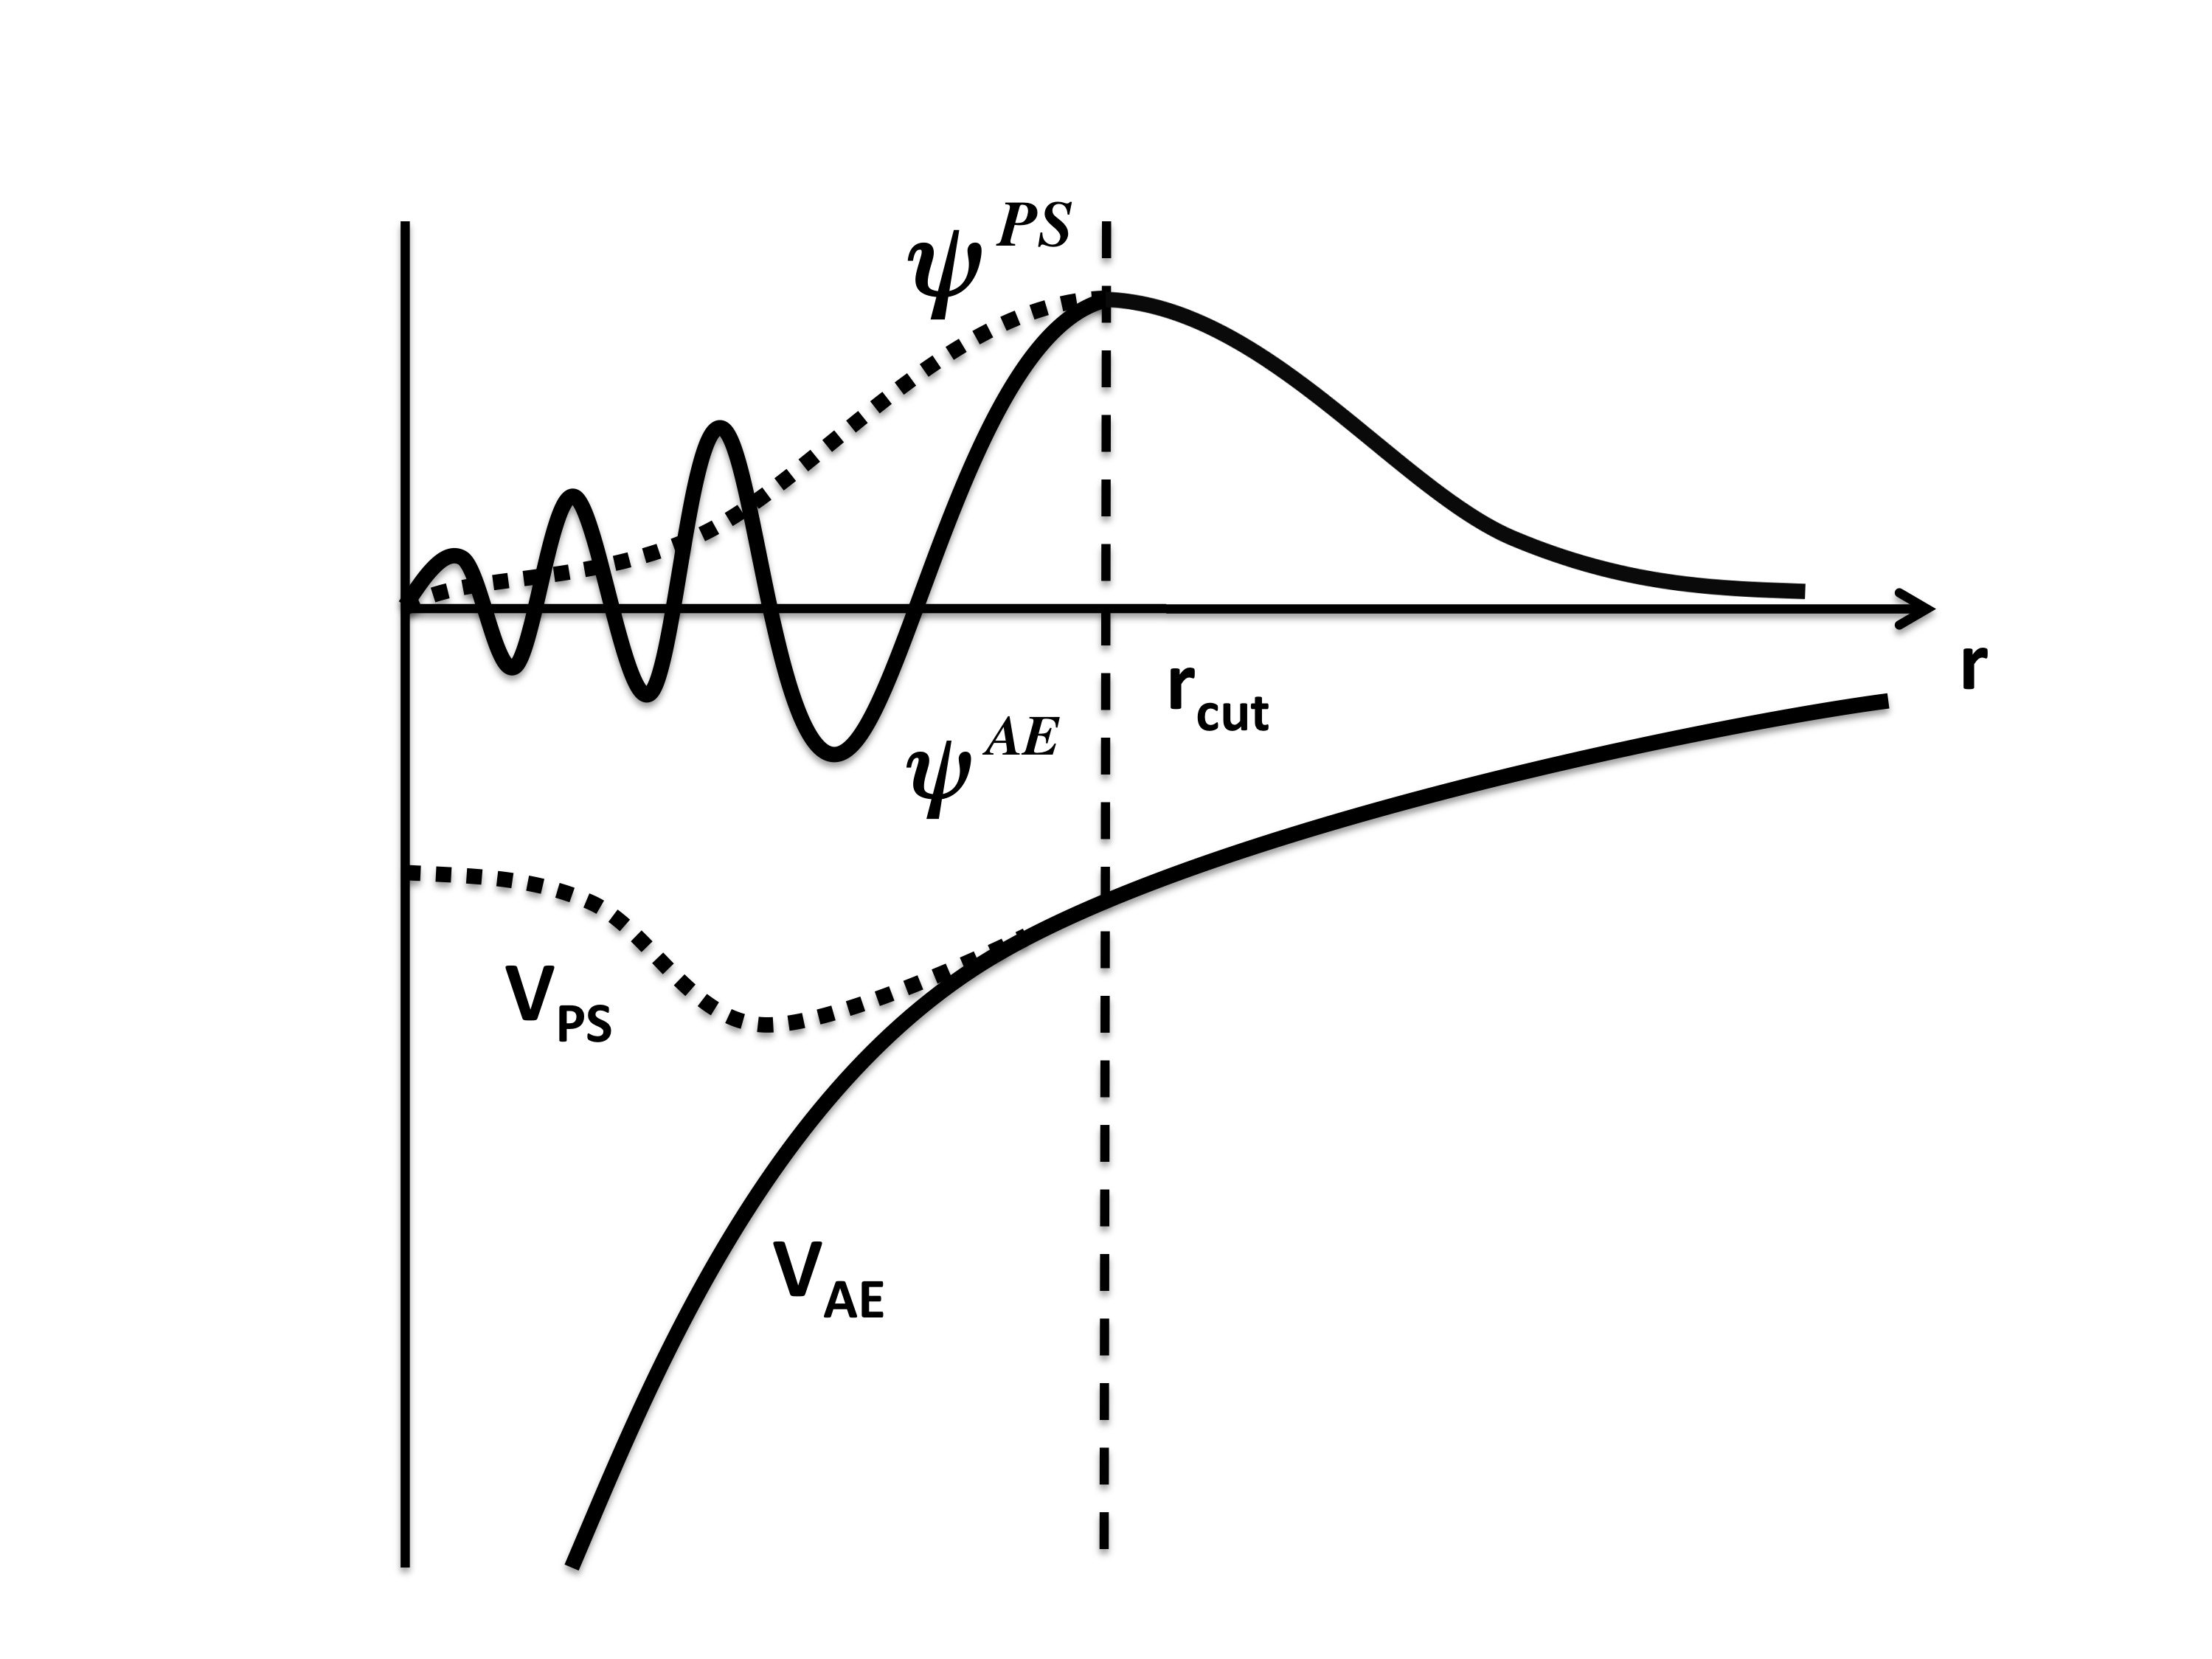
\includegraphics[height=10cm]{images/pseudopotential.png}
\end{center}
\caption[Sketch of an all-electron potential V$_{AE}$ and a pseudopotential V$_{PS}$ with their corresponding wave functions. r$_{cut}$ indicates the radius beyond which both the potentials and their wave functions are the same.]{Sketch of an all-electron potential V$_{AE}$ and a pseudopotential V$_{PS}$ with their corresponding wave functions. r$_{cut}$ indicates the radius beyond which both the potentials and their wave functions are the same. Adapted from \cite{Payne1992}.}
\label{figure:pseudopotential}
\end{figure}

Figures \ref{figure:o_pp} and \ref{figure:zr_pp} show the actual pseudopotentials used throughout this work for oxygen and zirconium respectively. The potentials are shown broken down by the electronic sub-shells occupied by the valence electrons. The pseudopotentials are shown in order of increasing sub-shell energies, thus the 5s electron orbitals are filled before the 4d orbitals in zirconium. Two lines for the all-electron wavefunction are shown, corresponding to the different electron angular momenta.

\begin{figure}[ht] % Oxygen pseudopotentials
\begin{center}
\begin{tikzpicture}
	\begin{groupplot}[group style={group size=1 by 2}, width=14cm, height=7cm]
	\nextgroupplot[
    axis y line*=middle, axis x line*=bottom, y label style={at={(-0.03,-0.1)}}, ylabel=Wavefunction $\Psi$, axis y line shift=0.5cm,
    xtick=\empty, ymin=-1.1, ymax=1.1, ytick={-1, -0.5, 0, 0.5, 1}, xmax=2.5, 
    x axis line style={white}]
         \addplot[no marks, dashed, draw=red!80!white] table [x=distance, y=O_AE_s1,]{dat/o_pp.dat}; 
		\addplot[no marks, draw=red!80!white] table [x=distance, y=O_pp_s1,]{dat/o_pp.dat}; 
		\addplot[no marks, dashed, draw=blue!80!white] table [x=distance, y=O_AE_s2,]{dat/o_pp.dat}; 
		\addplot[no marks, draw=blue!80!white] table [x=distance, y=O_pp_s2,]{dat/o_pp.dat};
		\node at (0.1, 0.99) {\textbf{O (2s)}};
		\draw[black] % horizontal line
				(-0.11, 0)
				-- % = line-to
				++ % = calculate a vector sum
				(axis direction cs:2.61, 0);
		\draw[black, dotted] % Vertical line
				(1.299,1)
				-- % = line-to
				++ % = calculate a vector sum
				(axis direction cs:0,-2);
				
    \nextgroupplot[
    axis y line*=middle, axis x line*=bottom, axis x line shift=0, x axis line style={white}, axis y line shift=0.5cm,
    ymin=-1.1, ymax=1.1, ytick={-1, -0.5, 0, 0.5, 1}, xtick={0, 0.5, 1, 1.5, 2, 2.5}, xmax=2.5, xlabel=Distance from nucleus (Bohr)]
         \addplot[no marks, dashed, draw=red!80!white] table [x=distance, y=O_AE_p1,]{dat/o_pp.dat}; 
		\addplot[no marks, draw=red!80!white] table [x=distance, y=O_pp_p1,]{dat/o_pp.dat}; 
		\addplot[no marks, dashed, draw=blue!80!white] table [x=distance, y=O_AE_p2,]{dat/o_pp.dat}; 
		\addplot[no marks, draw=blue!80!white] table [x=distance, y=O_pp_p2,]{dat/o_pp.dat}; 
		\node at (0.1, 0.99) {\textbf{O (2p)}};
		\draw[black] % horizontal line
				(-0.11, 0)
				-- % = line-to
				++ % = calculate a vector sum
				(axis direction cs:2.61, 0);
		\draw[black, dotted] % vertical line
				(1.299,1)
				-- % = line-to
				++ % = calculate a vector sum
				(axis direction cs:0,-2);
	\end{groupplot}
		\end{tikzpicture}
		\caption{Plots of the valence $s$ and $p$ orbital potentials for oxygen with two projectors per angular momentum. Dashed lines indicate the all-electron potentials while solid lines indicate the corresponding pseudopotential. Dotted vertical line marks the radius beyond which the potentials match.}
		\label{figure:o_pp}
	\end{center}
\end{figure}

\clearpage

\begin{figure}[h!] % Zirconium pseudopotentials
\begin{center}
\begin{tikzpicture}
	\begin{groupplot}[group style={group size=1 by 3}, width=14cm, height=7cm]
	\nextgroupplot[ % 4p
    axis y line*=middle, axis x line*=bottom, axis y line shift=0.5cm,
    xtick=\empty, ymin=-1.2, ymax=1.2, ytick={-1, -0.5, 0, 0.5, 1}, xmax=2.5, 
    x axis line style={white}]
         \addplot[no marks, dashed, draw=red!80!white] table [x=distance, y=Zr_AE_p1,]{dat/zr_pp.dat}; 
		\addplot[no marks, draw=red!80!white] table [x=distance, y=Zr_pp_p1,]{dat/zr_pp.dat}; 
		\addplot[no marks, dashed, draw=blue!80!white] table [x=distance, y=Zr_AE_p2,]{dat/zr_pp.dat}; 
		\addplot[no marks, draw=blue!80!white] table [x=distance, y=Zr_pp_p2,]{dat/zr_pp.dat};
		\node at (0.1, 0.99) {\textbf{Zr (4p)}};
		\draw[black] % horizontal line
				(-0.11, 0)
				-- % = line-to
				++ % = calculate a vector sum
				(axis direction cs:2.61, 0);
		\draw[black, dotted] % Vertical line
				(2.105,1)
				-- % = line-to
				++ % = calculate a vector sum
				(axis direction cs:0,-2);
				
	\nextgroupplot[ % 5s
    axis y line*=middle, axis x line*=bottom, axis y line shift=0.5cm, ylabel=Wavefunction $\Psi$,
    xtick=\empty, ymin=-1.2, ymax=1.2, ytick={-1, -0.5, 0, 0.5, 1}, xmax=2.5, 
    x axis line style={white}]
         \addplot[no marks, dashed, draw=red!80!white] table [x=distance, y=Zr_AE_s1,]{dat/zr_pp.dat}; 
		\addplot[no marks, draw=red!80!white] table [x=distance, y=Zr_pp_s1,]{dat/zr_pp.dat}; 
		\addplot[no marks, dashed, draw=blue!80!white] table [x=distance, y=Zr_AE_s2,]{dat/zr_pp.dat}; 
		\addplot[no marks, draw=blue!80!white] table [x=distance, y=Zr_pp_s2,]{dat/zr_pp.dat};
		\node at (0.1, 0.99) {\textbf{Zr (5s)}};
		\draw[black] % horizontal line
				(-0.11, 0)
				-- % = line-to
				++ % = calculate a vector sum
				(axis direction cs:2.61, 0);
		\draw[black, dotted] % Vertical line
				(2.105,1)
				-- % = line-to
				++ % = calculate a vector sum
				(axis direction cs:0,-2);
				
    \nextgroupplot[ % 4d
    axis y line*=middle, axis x line*=bottom, axis x line shift=0, x axis line style={white}, axis y line shift=0.5cm,
    ymin=-1.2, ymax=1.2, ytick={-1, -0.5, 0, 0.5, 1}, xtick={0, 0.5, 1, 1.5, 2, 2.5}, xmax=2.5, xlabel=Distance from nucleus (Bohr)]
         \addplot[no marks, dashed, draw=red!80!white] table [x=distance, y=Zr_AE_d1,]{dat/zr_pp.dat}; 
		\addplot[no marks, draw=red!80!white] table [x=distance, y=Zr_pp_d1,]{dat/zr_pp.dat}; 
		\addplot[no marks, dashed, draw=blue!80!white] table [x=distance, y=Zr_AE_d2,]{dat/zr_pp.dat}; 
		\addplot[no marks, draw=blue!80!white] table [x=distance, y=Zr_pp_d2,]{dat/zr_pp.dat}; 
		\node at (0.1, 0.99) {\textbf{Zr (4d)}};
		\draw[black] % horizontal line
				(-0.11, 0)
				-- % = line-to
				++ % = calculate a vector sum
				(axis direction cs:2.61, 0);
		\draw[black, dotted] % vertical line
				(2.105,1)
				-- % = line-to
				++ % = calculate a vector sum
				(axis direction cs:0,-2);
	\end{groupplot}
		\end{tikzpicture}
		\caption{Plots of the valence $s$, $p$ and $d$ orbital potentials for zirconium with two projectors per angular momentum. Dashed lines indicate the all-electron potentials while solid lines indicate the corresponding pseudopotential. Dotted vertical line marks the radius beyond which the potentials match.}
		\label{figure:zr_pp}
	\end{center}
\end{figure}

%\begin{figure}[ht] % Oxygen pseudopotential
%\begin{center}
%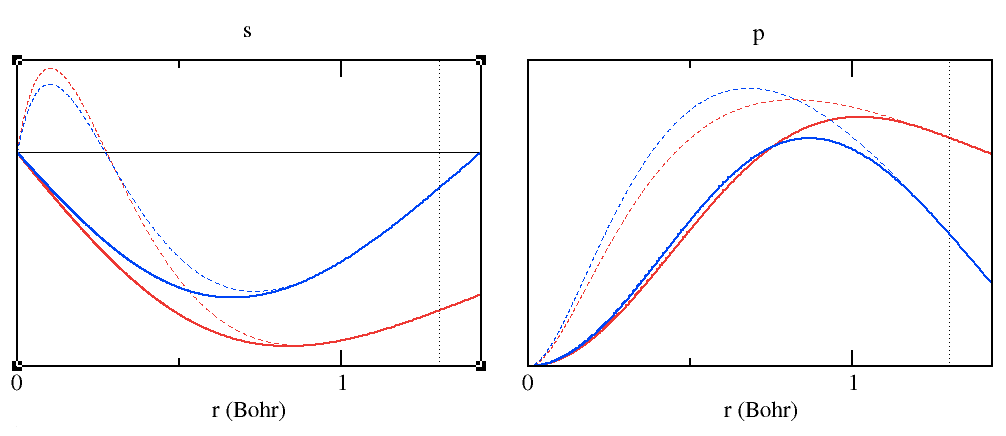
\includegraphics[height=7.3cm]{images/oxygen_otf_pp.png}
%\end{center}
%\caption{Plots of the valence $s$ and $p$ orbital potentials for oxygen with two projectors per angular momentum. Dashed lines indicate the all-electron potentials while solid lines indicate the corresponding pseudopotential. Dotted vertical line marks the radius beyond which the potentials match.}
%\label{figure:oxygen_pseudopotential}
%\end{figure}

%\begin{figure}[ht] % Zirconium pseudopotential
%\begin{center}
%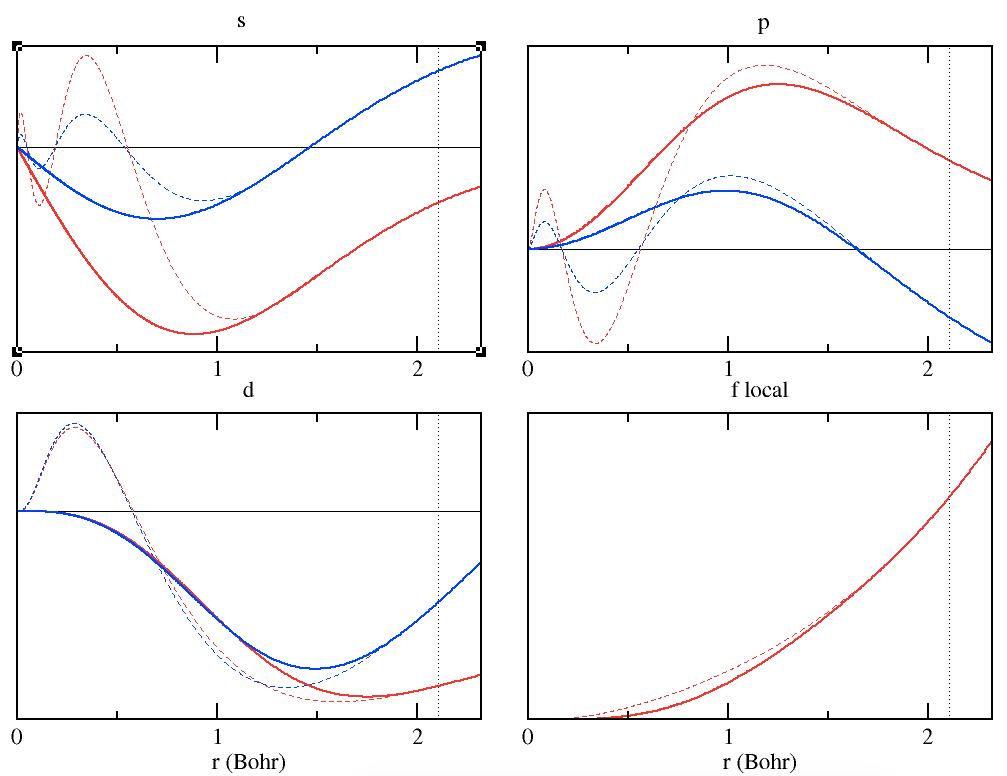
\includegraphics[height=12cm]{images/zirconium_otf_pp.png}
%\end{center}
%\caption{Plots of the valence $s$, $p$ and $d$ orbital potentials for zirconium with two projectors per angular momentum. Dashed lines show the all-electron potentials while solid lines indicate the corresponding pseudopotential. Dotted vertical line marks the radius beyond which the potentials match.}
%\label{figure:zirconium_pseudopotential}
%\end{figure}


\section{Periodic boundaries}

\subsection{Bloch's theorem}

The repeating nature of a crystal structure, defined by the lattice vectors plus a basis set of atoms that are repeated, is well-suited for computer models. It allows us to define periodicity in three dimensions for a given unit cell. An example of this periodicity is illustrated in Figure \ref{figure:periodicboundary} in two dimensions. A model based on this periodicity is justified as follows:

\begin{itemize}
\item Nuclei are arranged in a periodically repeating pattern, thus their potentials acting on electrons are also periodic.
\item If the potential is periodic, it follows that the electron density is also periodic.
\item The electron density is equivalent to the square of the wave function magnitude, thus the magnitude of the wave function is also periodic.
\end{itemize}

\begin{figure}[ht] % Periodic boundary image
\begin{center}
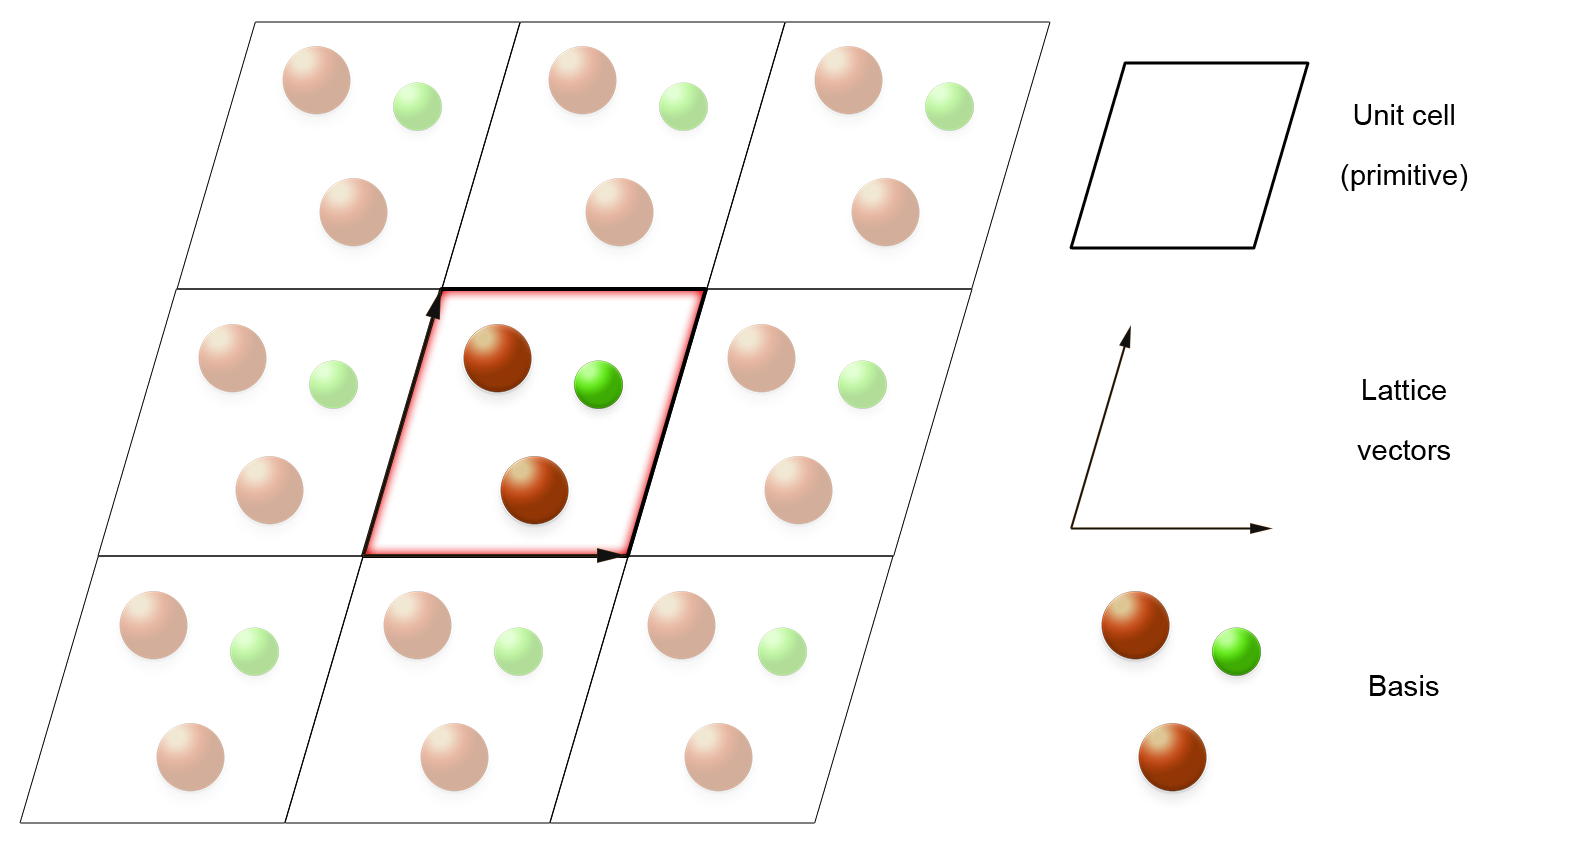
\includegraphics[width=\linewidth]{images/PeriodicBoundaryThesis.png}
\end{center}
\caption{Two dimensional illustration of periodic boundary around a primitive cell.}
\label{figure:periodicboundary}
\end{figure}

Knowing that the magnitude of the wave function is periodic greatly simplifies the calculation process; only one `period' of the function needs to be evaluated. However, the phase of the wave function can take any of an infinite number of values and still satisfy the periodicity condition. At this point, we consider Bloch's theorem which states that the possible wave functions are all quasi-periodic, and thus the wave function can be expressed as:  % Patrick's Fig 2.3 is really useful for describing this
\begin{equation}
\label{equation:bloch}
\psi_k(\textbf{r}) = e^{i\textbf{k}.\textbf{r}}u_k(\textbf{r})
\end{equation}

Where $\psi_k(\textbf{r})$ is the wave function evaluated at position \textbf{r}, $e^{i\textbf{k}.\textbf{r}}$ is an arbitrary phase factor, and $u_k(\textbf{r})$ is a periodic function with the same periodicity as the wave function. Solutions to this equation exist for any value of \textbf{k} and so the general solution can be expressed as an integral over the first Brillouin zone, the primitive lattice cell in reciprocal space. Instead of evaluating the integral over the range of \textbf{k} (a computationally costly task as it is done for many wave functions), a sum of values at discrete points, known as \textbf{k}-points, is used. This approximation is valid because the wave function varies slowly over \textbf{k}, thus allowing the integral to be approximated with several appropriately spaced \textbf{k}-points. In general, a finer \textbf{k}-point grid results in increased accuracy, but at an increased computational cost \cite{Hasnip2010}. For all DFT calculations in this thesis, a Monkhorst-Pack sampling scheme \cite{Monkhorst1976} was used for Brillouin zone integration, with a minimum \textbf{k}-point separation of 0.09 \r{A}$^{-1}$.

\subsection{Plane-waves}

The electron density of a system is described in the context of a basis set. A basis set is a collection of functions (known as basis functions) which can be combined to produce some relevant output, typically the mathematical description for the shape of an electron orbital. For example, any sound wave can be generated from a combination of sine functions (basis functions). 

The purpose of a basis set in DFT calculations is to describe the varying amplitude of the electron density in space. Any complete basis set (e.g. plane-wave, correlation-consistent, split-valence) may be used to represent the behaviour of electron orbitals, but a plane-wave method was chosen due to its greater suitability for periodic systems (plane-waves are intrinsically periodic). Since the electron densities are represented by a finite sum of plane-waves with different energies, a truncation error will be incurred. Plane-waves of higher energies provide a smaller contribution to the overall density, so only plane-wave up to a chosen cut-off energy value are considered in order to reduce computational requirements. An appropriate plane-wave cut-off energy must therefore be determined through a convergence test. 

%Figure \ref{Figure:cutoffconvergence} shows the first convergence study where the total energy of simulations with various values of $E_{cutoff}$ were compared to a highly converged value, and then plotted on a log scale to see how precision is improved at larger values.


\section{Computational details}
\subsection{Cell dimensions and initialisation}

A supercell method is used for the study of various defects. The first step is to create a unit cell of \zirconia\ in each of the three crystal structures. Each unit cell is then fully relaxed through a geometry optimisation process (see § \ref{geometry_optimisation_method}). The resulting cell is used to construct supercells through tessellation in three dimensions, before being fully relaxed again. In this way, we generate systems with up to ten times as many atoms as the unit cell (supercell details can be found in Table \ref{table:supercells}). This is necessary because introducing defects into a small unit cell will result in the defect interacting with itself across the periodic boundary. A supercell increases the distance between the defect and its periodic image, using the bulk material as an interaction buffer. 

When constructing a supercell, it is important to consider making the supercell equally large in all directions, such that any directional bias in defect-defect interaction is minimised. Larger supercells carry an increased computational cost when running calculations, limiting the sizes we can achieve. For example, a constant-volume defect calculation with 300 atom supercells will take upwards of 500 hours to complete (on the Imperial College HPC using four 32-core nodes), whereas the equivalent 100 atom supercell will take just 72 hours (fully relaxed calculations are even more computationally expensive).


\begin{table}[ht] % Supercell details
\doublespacing
\centering
\caption{Composition of the supercells in terms of the number of individual unit cells stacked in each direction.} % Unit cells were stacked in such a way as to produce the most cubic supercell in order to minimise directional defect-defect interactions.}
\vspace*{2mm}
\label{table:supercells}
\begin{tabular}{cccccccc}
\hline
\multirow{2}{*}{{\bf \begin{tabular}[c]{@{}c@{}}Crystal \\ Structure\end{tabular}}} & \multicolumn{3}{c}{{\bf No. unit cells}} & \multicolumn{3}{c}{{\bf Supercell size (\AA)}} & \multirow{2}{*}{{\bf \begin{tabular}[c]{@{}c@{}}No.\\ atoms\end{tabular}}} \\ \cline{2-7}
 & \hspace{0.25 cm} a \hspace{0.2 cm} & b & c & a \hspace{0.0 cm} & b & c \hspace{0.35 cm} &  \\ \hline
\begin{tabular}[c]{@{}c@{}}Monoclinic\\ ($P2_1/c$)\end{tabular} & 2 & 2 & 2 & 10.37 & 10.47 & 10.75 & 96 \\ \hline
\begin{tabular}[c]{@{}c@{}}Tetragonal\\ ($P4_2/nmc$)\end{tabular} & 3 & 3 & 2 & 10.85 & 10.85 & 10.56 & 108 \\ \hline
\begin{tabular}[c]{@{}c@{}}Cubic\\ ($Fm\overline{3}m$)\end{tabular} & 2 & 2 & 2 & 10.22 & 10.22 & 10.22 & 96 \\ \hline
\end{tabular}
\end{table}

\subsection{Geometry optimisation} \label{geometry_optimisation_method}

The geometry optimisation task in CASTEP follows a simple steepest-descent algorithm which attempts to satisfy certain convergence criteria, depending on the constraints applied to the system. This is an iterative process which takes an initial system state, modifies ion positions slightly and then calculates the difference in properties between the states to check for convergence. 

The variational principle in quantum mechanics tells us that the lowest system energy calculated is always an upper bound for the ground state energy, thus providing a way to check if modifications to the system are actually optimising the geometry. The exception is when the system converges upon a local minima, which may not be an experimentally observed state. This can be avoided to some extent by having good initial ion placement from which to optimise.

\subsection{Convergence criteria for geometry optimisation} \label{convergence_criteria}

Four convergence criteria are used for the geometry optimisation tasks throughout this work, one of which is only used when performing constant-pressure calculations, such as when a supercell is being fully relaxed. These criteria are evaluated with respect to the previous iteration during the geometry optimisation task:

\begin{itemize}
\item \emph{Change in energy per ion}: The largest change in the energy per ion between iterations must be below $10^{-5}$ eV. Below this value, the total energy improvement towards the ground state for a 100 atom supercell is less than 0.001 eV, and is therefore considered converged.
\item \emph{Maximum force on an ion}: The maximum force requirement on any single ion in an iteration must be below $10^{-2}$ eV/\r{A}. This is required to make sure that the ion position will not change significantly in the following iteration, possibly bringing another convergence criterion above its threshold.
\item \emph{Maximum change in ion position}: This must be below $5 \times 10^{-4}$ \r{A} between iterations to be considered converged. This criterion specifies the maximum `rattle' of the ion that is tolerated once the minimum energy is reached (i.e. displacements above this value may still be important for achieving a correct atomic configuration). 
\item \emph{Maximum stress (constant-pressure only)}: During unconstrained relaxation, the maximum change in stress between iterations should be below 50 MPa. This is necessary to avoid large deviations which may distort the symmetry of the supercell, resulting in anomalous energy values.
\end{itemize}

Using these convergence criteria, non-defective supercells of \zirconia\ were relaxed under constant pressure. The resulting structure was used as the starting point to which defects were introduced, and subsequently relaxed again, this time under constant volume conditions to simulate low defect concentrations \cite{Murphy2014, Bell2015}. Finally, all DFT calculations on doped and defective structures in this thesis employed the Pulay method for density mixing \cite{Pulay1980} to take into consideration changes in electronic behaviour of the system caused by the defect.

\subsection{Charged cell correction} \label{charged_cell_correction}

When calculating the energy of a defect with an overall non-zero charge, this charge introduces a systematic error in the energy value which is a function of the charge magnitude. This is typically the case in high band-gap materials such as \zirconia\ where electron mobility is far lower than in metals or semiconductors, allowing defects such as \ch{V_{O}^{**}} and \ch{V_{Zr}^{''''}} to be thermodynamically stable in the lattice. 

The source of the error from charged defects is self-interaction across the periodic boundary, made necessary by the finite cell size. A common solution is to append a Makov-Payne correction term when calculating formation energies of defects \cite{Makov1995, Makov1996}. This works well in many cases, but does not take into consideration the anisotropy in the material's dielectric properties, as is the case in tetragonal \zirconia\ due to the non-unity lattice $c/a$ ratio. These effects are better captured when using a screened Madelung correction \cite{Murphy2013}. This method provides a more complete description of the dielectric properties by utilising a dielectric tensor rather than a single value of the dielectric constant (or relative permittivity). Dielectric tensors for the different phases of \zirconia\ were taken from \cite{Zhao2002a, Zhao2002}. The screened Madelung correction is therefore used in preference to a Makov-Payne correction throughout this thesis.

\subsection{Helmholtz free energy} \label{helmholtz_method}

In order to examine the relationship between temperature and energy for the different \zirconia\ phases, phonon calculations were performed in CASTEP using a method outlined by Burr \emph{et al.} \cite{burr2015crystal,jackson2016resolving}. This entails using the harmonic approximation to determine the shape of the potential well that an atom sits in. The potential well is approximated by a spherically symmetric harmonic well, centred at an atom's equilibrium position in the lattice. At a temperature of 0 K, an atom will occupy the lowest region of its potential well, known as the ground state (though they will still have energy, known as zero-point energy). As temperature increases, the atom will sometimes occupy higher energy states in the potential well due to increased thermal vibrations, moving from its equilibrium position. The total energy ($A(T, V)$) of this system, known as the Helmholtz free energy, is calculated using the internal energy ($U(V)$), vibrational enthalpy ($H_{v}(T, V)$), vibrational entropy ($S_{v}(T, V)$) and configurational entropy ($S_{conf}$):
\begin{equation} \label{vibrational}
A(T, V) = U(V) + H_{v}(T, V) - TS_{v}(T, V) - TS_{conf} 
\end{equation}
where $T$ is temperature and $V$ is volume. The configurational entropy is calculated using Boltzmann statistics:
\begin{equation}
S_{conf} = k_{B}\ch{ln}(\Omega)
\end{equation}
where $k_{B}$ is the Boltzmann constant and $\Omega$ denotes the number of possible configurations (i.e. valid permutations of energy level occupancy). The vibrational terms in Equation \ref{vibrational} are obtained by performing a constant-volume phonon calculation in CASTEP and then integrating over the resulting phonon DOS. This is done over a range of temperatures for each crystal structure of \zirconia .

\subsection{Incorporation energies}

The inner oxide of the fuel cladding will be highly defective due to radiation damage, resulting in a high concentration of pre-existing intrinsic defect sites relative to the concentration of fission products. We therefore consider the energy of fission product incorporation on to these existing defect sites. The energies to incorporate atoms at interstitial and substitutional sites in \zirconia\ were calculated from the set of defective and perfect supercell DFT energies. For iodine, incorporation energies were established to place atoms into vacancy sites of different charge to generate defects from \ch{I_{O}^{x}} to \ch{I_{O}^{**}}, and \ch{I_{Zr}^{x}} to \ch{I_{Zr}^{''''}}. I was also incorporated onto the interstitial sites.

The incorporation energy equation for iodine uses $\frac{1}{2}$I$_{2}$ as the reference state of iodine, while Te, Xe and Cs use the DFT energy calculated as a single atom in a large cell:
\begin{equation}
\label{interstitial_incorp_equation}
E_{inc}(\ch{I_{$i$}^{x}}) = E_{DFT}(\ch{I_{$i$}^{x}}) - (E_{DFT}(ZrO_2) + \frac{1}{2}\mu_{I_{2}})  % - \frac{E_{I_2}}{2}
\end{equation}
where $E_{inc}(\ch{I_{$i$}^{x}})$ is the incorporation energy of a neutral iodine interstitial, $E_{DFT}(\ch{I_{$i$}^{x}})$ is the energy of a neutral iodine interstitial, $E_{DFT}(ZrO_2)$ is the energy of a non-defective \zirconia\ supercell and $\mu_{I_{2}}$ is the chemical potential of an I$_{2}$ molecule, taken from a single point DFT calculation of the I$_{2}$ dimer. For incorporation of a charged interstitial (e.g. $\ch{I_{i}^{*}}$), the energy required to add or remove an electron is included in the calculation:
\begin{equation}
\label{interstitial_incorp_equation_charged}
E_{inc}(\ch{I_{$i$}^{n}}) = E_{DFT}(\ch{I_{$i$}^{n}}) - (E_{DFT}(ZrO_2) + \frac{1}{2}\mu_{I_{2}} + n(E_{VBM} + \mu_{e}))
\end{equation}
Similarly, for a substitutional defect:
\begin{equation}
\label{o_sub_incorp_equation}
E_{inc}(\ch{I_{O}^{$n$}}) = E_{DFT}(\ch{I_{O}^{$n$}}) - (E_{DFT}(\ch{V_{O}^{$n$}}) + \frac{1}{2}\mu_{I_{2}})  % - \frac{E_{I_2}}{2}
\end{equation}
where $\ch{I_{O}^{$n$}}$ is an iodine substitutional defect at an oxygen site of charge $n$ and $\ch{V_{O}^{$n$}}$ is the corresponding oxygen vacancy.

\subsection{Stiffness matrix generation}

The elastic stiffness matrices for the pure monoclinic, tetragonal and cubic phases of \zirconia\ were calculated using CASTEP's \emph{elastic constants} task. The calculation of elastic constants is a multi-step process involving up to 36 individual DFT calculations. Several scripts have been made available to simplify this process (see Appendix \ref{castep_scripts}).

The first step is to generate multiple different \texttt{.cell} files, each with either a small deviation in the lattice parameter or an additional shear on the cell. This requires starting with a unit cell that has already been completely relaxed via the \emph{geometry optimisation} task. In total, 36 \texttt{.cell} files are generated, each corresponding to a single element of the eventual stiffness matrix. The next step is to run a single point DFT calculation on each \texttt{.cell} file with the \emph{calculate stress} parameter enabled to output the resulting stress matrix. The final step is to use Hooke's Law to calculate the elastic stiffness constants using the known stress and strain state. 

%\subsection{Strain method for defect volumes}
%
%The volumes of the defective supercells were kept constant because constant pressure calculations have been shown to sometimes break the symmetry of the supercell \cite{samanta2010thermodynamic}, leading to unreliable energy values. This is partly due to the assumed arrangement of the defects that may not be commensurate with the cell symmetry. This approach to calculating defect volumes then relies on calculating the elastic constants of the non-defective supercell, followed by extracting the resultant stress tensor from a defect simulation. The strain tensor of the defective cell can then be calculated using Hooke's law, giving the relaxation volume. 

\subsection{Defect relaxation volumes} \label{isobaricmethod}

Defect relaxation volumes of point defects were calculated using an isobaric method, requiring two calculations to be performed under constant-pressure using the geometry optimisation task in CASTEP. The defect relaxation volume ($\Delta$V) is defined as: 
\begin{equation}
\Delta V = V_{def} - V_{perf}
\end{equation}
where $V_{def}$ is the relaxation volume of the defective supercell and $V_{perf}$ is the relaxation volume of the non-defective (perfect) supercell. In this thesis, mentions of `volume' will refer to relaxation volumes unless stated otherwise.

After completing an energy calculation, CASTEP provides the volume of the resulting cell, defined as the space enclosed by the repeating unit of atoms within the calculated lattice parameters. By subtracting the volume of a non-defective cell from the volume of a defective cell, we obtain a value for the total defect volume. 

It is important to consider that if there is a non-zero charge on the system, this will affect the calculated volume. Two systems with the same type, amount and arrangement of atoms, but different overall charges, will have different energies (due to the number of electrons). Different electronic orbital occupancies will affect the inter-atomic forces and therefore the shape of the cell. In order to compensate for this effect, a `corrected' relaxation volume, as described by Goyal \emph{et al.} is calculated when the defect has a non-zero charge:
\begin{equation}
\Delta V = V_{def}^{q} - V_{perf}^{q}
\end{equation}
where $q$ is the defect charge. This formulation uses the volume of a non-defective supercell with equal charge magnitude as the reference structure. This method has been shown to yield more reasonable defect volumes than when using neutral non-defective supercells as the reference structure \cite{goyal2017conundrum}. Defect volumes without this correction applied are provided in Appendix \ref{uncorrected_volumes} for comparison.

\section{Defect energies and equilibria} 

\subsection{Defect formation energies}

Defect formation energies are calculated using equation \ref{equation:formation_energy}:
\begin{equation} \label{equation:formation_energy}
    E_{f} = E_{def} - (E_{perf} \pm \sum_{i} n_i\mu_i + q(E_{VBM} + \mu_{e})) + E_{corr}
\end{equation}
where $E_{f}$ is the formation energy, $E_{def}$ is the energy of the defective supercell, $E_{perf}$ is the energy of a non-defective supercell, $q$ is the defect charge, $E_{VBM}$ is the valence band maximum, $\mu_{e}$ is the Fermi level relative to the VBM and $E_{corr}$ is a charged-cell correction term (see § \ref{charged_cell_correction}). Since $\mu_{e}$ is not a fixed value, plots of formation energy against $\mu_{e}$ are produced to examine the behaviour of defects across the entire range of the band gap. These are reported in Figures \ref{figure:monovacancies}, \ref{figure:tetvacancies} and \ref{figure:cubicvacancies}.

\subsection{Defect equilibria} \label{brouwer_method} % 

Typically in materials, several types of defects will exist simultaneously. These defects will be present at an equilibrium concentration based on their thermodynamic stability. Predicting the defect equilibria is possible with statistical mechanics and some approximations. For example, it is expected that a crystal lattice will usually be overall charge-neutral (exceptions can be made under certain conditions, see § \ref{space_charge}), otherwise we would see a build-up of charge with a large Coulomb energy penalty which would be thermodynamically unsustainable.

Brouwer diagrams, also known as Kr{\"o}ger-Vink diagrams, were produced using a method outlined by Murphy et al. \cite{Murphy2014, Murphy2014a} through which it is possible to determine defect concentrations as a function of oxygen partial pressure. We start from the statement that the chemical potential of \zirconia\ is equivalent to the sum of chemical potentials $\mu$ of its constituent species, Zr and O:
\begin{equation}
{\mu}_{ZrO_2(s)} = {\mu}_{Zr}(p_{O_2}, T) + {\mu}_{O_{2}}(p_{O_{2}}, T)
\label{mewZrO2compmethodology}
\end{equation}
where $T$ denotes temperature and $p_{O_2}$ denotes oxygen partial pressure. The chemical potential of \zirconia\ in the solid state is assumed to have negligible dependence on $T$ and $p_{O_2}$ relative to ${\mu}_{Zr}$ and ${\mu}_{O_2}$. Energies can be obtained for bulk \zirconia\ and Zr, but the ground state of oxygen is not correctly reproduced in DFT \cite{Batyrev2000,Lozovoi2001}. Instead, we use the approach of Finnis et al. \cite{Finnis2005} to infer the oxygen chemical potential from standard state values. We can use the experimental Gibbs free energy to produce an equation where $\mu_{O_2}$ is the only unknown:
\begin{equation}
\Delta{G^{\plimsoll}_{f, ZrO_2}} = \mu_{ZrO_2(s)} - (\mu_{Zr(s)} + \mu^{\plimsoll}_{O_2})
\end{equation}
where $\Delta{G^{\plimsoll}_{f, ZrO_2}}$ is the experimental Gibbs energy at standard temperature and pressure and $\mu^{\plimsoll}_{O_2}$ is the oxygen chemical potential under the same conditions. Only monoclinic \zirconia\ is stable under standard conditions, with $\Delta{G^{\plimsoll}_{f, ZrO_2}}$ = -1042.746 kJ/mol (10.807 eV) \cite{brown2005chemical}. Values of the Gibbs free energy of formation for the tetragonal (10.697 eV) and cubic (10.595 eV) phases were obtained by adding the energy difference between the phases from DFT calculations. The values of $\mu_{ZrO_2(s)}$ and $\mu_{Zr(s)}$ are calculated using DFT. Once $\mu^{\plimsoll}_{O_2}$ is calculated, we can generalise the chemical potential of oxygen for any value of $T$ and $p_{O_2}$ by appending an ideal gas relationship $\Delta{\mu(T)}$ and a Boltzmann distribution:
\begin{gather}
\mu_{O_2}(p_{O_2},T) = \mu^{\plimsoll}_{O_2} + \Delta{\mu(T)} + \frac{1}{2}{k_B}log(\frac{p_{O_2}}{p^{\plimsoll}_{O_2}}) \\
\Delta \mu(T) = -\frac{1}{2}(S^{\plimsoll}_{O_{2}}- C^{\plimsoll}_{p})(T-T^{\plimsoll}) + C^{\plimsoll}_{p}T\textup{log}\left ( \frac{T}{T^{\plimsoll}} \right )
\end{gather} 
where $S^{\plimsoll}_{O_{2}}$ is the molecular entropy at standard temperature and pressure (T$^{\plimsoll}$ = 273.15 K, P$^{\plimsoll}$ = $10^{5}$ Pa), and $C^{\plimsoll}_{p}$ is the constant pressure heat capacity of oxygen. These quantities have values of $S^{\plimsoll}_{O_{2}}$ = 0.0021 eV/K and $C^{\plimsoll}_{p}$ = 0.000302 eV/K \cite{weast1984crc}. 

Using our generalised formula for $\mu_{O_2}$, we fix the temperature within the range of thermal phase-stabilisation (e.g. 1500 K for tetragonal \zirconia) and calculate $\mu_{O_2}$ for many different values of $p_{O_2}$ between $10^{-35}$ and 10$^{0}$ atm, corresponding to oxygen deficient and oxygen rich environments, respectively ($p_{O_2}$ in air is approximately 0.2 atm). While the tetragonal phase will be stress-stabilised in practice, thermal-stabilisation in such models has been shown to qualitatively approximate the effect of stress-stabilisation, while allowing a wider range of dopant behaviours to be predicted \cite{Bell2016}. 

Once a value of $\mu_{O_2}$ is calculated, defect concentrations can then be calculated using Boltzmann statistics. These concentrations were calculated using the method outlined by Kasamatsu \emph{et al}. whereby the effect of defects competing for the same lattice site is taken into account \cite{Kasamatsu2012}. The next step is to calculate the concentration of electron and hole defects. This is done by using the charge-neutrality condition to determine the Fermi level (electrochemical potential) in the system:
\begin{equation}
\sum_{i}q_{i}c_{i} - N_{c}\textrm{exp}{(-\frac{E_{g}-\mu_{e}}{k_{B}T})} + N_{v}\textrm{exp}{(-\frac{\mu_{e}}{k_{B}T})} = 0
\label{charge_neutrality}
\end{equation}

Where $c_{i}$ is the concentration of defect $i$, $q_{i}$ is its respective charge, $N_{c}$ and $N_{v}$ are the integrated density of states for the conduction and valence bands, $E_{g}$ is the band gap and $\mu_{e}$ is the Fermi level. 

\subsubsection{Temperature and pressure stabilisation}

As discussed in Chapter \ref{ch:crystallography}, the tetragonal and cubic phases are stabilised at elevated temperatures and pressures. However, DFT calculations of supercells under stress require significantly greater computational resources to yield sufficiently converged energy results, and so all DFT calculations in this thesis are performed on relaxed supercells. To account for this lack of stress stabilisation, Brouwer diagrams are generated at higher temperatures (where the tetragonal and cubic phases are thermally stabilised) rather than at 650 K, which is the expected temperature at the internal surface of the cladding. This approach to compensating for stress stabilisation follow that of similar studies published by other groups \cite{youssef2012intrinsic, Youssef2014, Otgonbaatar2014}.

\subsection{Effect of space charge} \label{space_charge}

Electrons have a higher rate of diffusion than oxygen vacancies in ZrO2, leading to a build-up of oxygen vacancies near the metal-oxide interface as corrosion progresses \cite{bojinov2010influence}. In the case of \zirconia , this effect will be pronounced because the layer is thin. This results in an overall positive charge (since the dominant oxygen vacancy is \ch{V_{O}^{**}}) referred to as a space charge. This effect can be taken into account when generating Brouwer diagrams by assuming an overall charge in the crystal structure instead of charge-neutrality:
\begin{equation}
\sum_{i}q_{i}c_{i} - N_{c}\textrm{exp}{(-\frac{E_{g}-\mu_{e}}{k_{B}T})} + N_{v}\textrm{exp}{(-\frac{\mu_{e}}{k_{B}T})} = q_{s}c_{s}
\label{charge_non_neutrality}
\end{equation}
where $q_{s}$ is the charge of a unit of the artificial space charge defect and $c_{s}$ is the concentration.

Figure \ref{figure:spacechargeexample} shows an example of the defect equilibria in tetragonal \zirconia\ with an overall positive space charge. In order for such a condition to be satisfied, higher concentrations of positively charged oxygen vacancy and hole defects are predicted to be present, while zirconium vacancy defects fall significantly. When extrinsic defects are also present in the lattice in significant concentrations, the space charge condition may influence which defect types are dominant at different oxygen pressures, as different oxidation states may be necessary to satisfy the charge condition.

%Another effect considered was the space charge of the system. Electrons have a higher rate of diffusion than oxygen vacancies in ZrO2, leading to a build-up of oxygen vacancies near the metal-oxide interface as corrosion progresses [44]. This results in an overall positive charge (since the dominant oxygen vacancy is referred to as a space charge. When included in our Brouwer diagrams, this space charge had a negligible effect on the concentration or charge state of iodine up to a charge of  holes per f.u. ZrO2. This corresponds to a high concentration of oxygen vacancies relative to the equilibrium concentration, predicting that a significant deviation from the equilibrium is not expected near the metal oxide interface as a result of a positive space charge.

\begin{figure}[htp] % Tet intrinsic no space charge
\begin{center}
\begin{tikzpicture}
	\begin{groupplot}[group style={group size=1 by 2}, width=14cm, height=11cm]
	\nextgroupplot[
		 ylabel={\ch{log_{10}}([D]) (per f.u.)}, ymin=-10, ymax=0, xmin=-35, xmax=0, legend style={{draw=}, at={(0.40,0.97)}, anchor=north west, legend columns=2, nodes={scale=1, transform shape}}]
        \addplot[no marks, draw=blue!70!black] table [x=pO2, y=electrons,]{dat/intrinsic_tet.dat}; \addlegendentry{\ch{e^{'}}}; \node at (-26.0,-2) {\ch{e^{'}}};
        \addplot[no marks, draw=red!85!black] table [x=pO2, y=holes,]{dat/intrinsic_tet.dat}; \addlegendentry{\ch{h^{\textperiodcentered}}}; \node at (-6.8,-3.6) {\ch{h^{\textperiodcentered}}};
        \addplot[no marks, draw=black!70!green] table [x=pO2, y=VO{2},]{dat/intrinsic_tet.dat}; \addlegendentry{\ch{V_{O}^{\textperiodcentered\textperiodcentered}}}; \node at (-28,-3) {\ch{V_{O}^{\textperiodcentered\textperiodcentered}}};
%         \addplot[no marks, draw=black!55!green] table [x=pO2, y=VO{1},]{dat/intrinsic_tet.dat}; \addlegendentry{\ch{V_{O}^{*}}};
%         \addplot[no marks, draw=black!30!green] table [x=pO2, y=VO{0},]{dat/intrinsic_tet.dat}; \addlegendentry{\ch{V_{O}^{x}}};
        \addplot[no marks, draw=yellow!85!blue] table [x=pO2, y=VM{-4},]{dat/intrinsic_tet.dat}; \addlegendentry{\ch{V_{Zr}^{''''}}}; \node at (-2.9,-4.6) {\ch{V_{Zr}^{''''}}};
%         \addplot[no marks, draw=yellow!75!blue] table [x=pO2, y=VM{-3},]{dat/intrinsic_tet.dat}; \addlegendentry{\ch{V_{Zr}^{'''}}};
%         \addplot[no marks, draw=yellow!65!blue] table [x=pO2, y=VM{-2},]{dat/intrinsic_tet.dat}; \addlegendentry{\ch{V_{Zr}^{''}}};
%         \addplot[no marks, draw=yellow!55!blue] table [x=pO2, y=VM{-1},]{dat/intrinsic_tet.dat}; \addlegendentry{\ch{V_{Zr}^{'}}};
%         \addplot[no marks, draw=yellow!45!blue] table [x=pO2, y=VM{0},]{dat/intrinsic_tet.dat}; \addlegendentry{\ch{V_{Zr}^{x}}};
%         \addplot[no marks, draw=red!60!yellow] table [x=pO2, y=Oi{-2},]{dat/intrinsic_tet.dat}; \addlegendentry{\ch{O_{i}^{''}}};
%         \addplot[no marks, draw=red!50!yellow] table [x=pO2, y=Oi{-1},]{dat/intrinsic_tet.dat}; \addlegendentry{\ch{O_{i}^{'}}};
%         \addplot[no marks, draw=red!40!yellow] table [x=pO2, y=Oi{0},]{dat/intrinsic_tet.dat}; \addlegendentry{\ch{O_{i}^{x}}};
%         \addplot[no marks, draw=green!80!pink] table [x=pO2, y=Mi{4},]{dat/intrinsic_tet.dat}; \addlegendentry{\ch{Zr_{i}^{****}}};
%         \addplot[no marks, draw=green!70!pink] table [x=pO2, y=Mi{3},]{dat/intrinsic_tet.dat}; \addlegendentry{\ch{Zr_{i}^{***}}};
%         \addplot[no marks, draw=green!60!pink] table [x=pO2, y=Mi{2},]{dat/intrinsic_tet.dat}; \addlegendentry{\ch{Zr_{i}^{\textbf{**}}}};
%         \addplot[no marks, draw=green!50!pink] table [x=pO2, y=Mi{1},]{dat/intrinsic_tet.dat}; \addlegendentry{\ch{Zr_{i}^{*}}};
%         \addplot[no marks, draw=green!40!pink] table [x=pO2, y=Mi{0},]{dat/intrinsic_tet.dat}; \addlegendentry{\ch{Zr_{i}^{x}}};
%         \addplot[no marks] table [x=pO2, y=Stoich,]{dat/intrinsic_tet.dat}; \addlegendentry{Stoich};
\node at (-33.7,-0.5) {\textbf{a)}}; 
			%\end{axis}     
%\end{tikzpicture}
%\begin{tikzpicture} % 1e-1
	\nextgroupplot[
		 xlabel={\ch{log_{10}}($p_{O_{2}}$) (atm)}, ylabel={\ch{log_{10}}([D]) (per f.u.)}, ymin=-10, ymax=0, xmin=-35, xmax=0, legend style={{draw=}, at={(0.40,0.97)}, anchor=north west, legend columns=4, nodes={scale=1, transform shape}}]
        \addplot[no marks, draw=blue!70!black] table [x=pO2, y=electrons,]{dat/intrinsic_spacecharge01.dat}; \node at (-26.5,-2.5) {\ch{e^{'}}};
        \addplot[no marks, draw=red!85!black] table [x=pO2, y=holes,]{dat/intrinsic_spacecharge01.dat}; \node at (-13,-3) {\ch{h^{\textperiodcentered}}};
        \addplot[no marks, draw=black!70!green] table [x=pO2, y=VO{2},]{dat/intrinsic_spacecharge01.dat}; \node at (-28,-0.8) {\ch{V_{O}^{\textperiodcentered\textperiodcentered}}};
%         \addplot[no marks, draw=black!55!green] table [x=pO2, y=VO{1},]{dat/intrinsic_spacecharge01.dat}; \addlegendentry{\ch{V_{O}^{*}}};
%         \addplot[no marks, draw=black!30!green] table [x=pO2, y=VO{0},]{dat/intrinsic_spacecharge01.dat}; \addlegendentry{\ch{V_{O}^{x}}};
        %\addplot[no marks, draw=yellow!85!blue] table [x=pO2, y=VM{-4},]{dat/intrinsic_spacecharge01.dat}; \node at (-3,-3) {\ch{V_{Zr}^{''''}}};
%         \addplot[no marks, draw=yellow!75!blue] table [x=pO2, y=VM{-3},]{dat/intrinsic_spacecharge01.dat}; \addlegendentry{\ch{V_{Zr}^{'''}}};
%         \addplot[no marks, draw=yellow!65!blue] table [x=pO2, y=VM{-2},]{dat/intrinsic_spacecharge01.dat}; \addlegendentry{\ch{V_{Zr}^{''}}};
%         \addplot[no marks, draw=yellow!55!blue] table [x=pO2, y=VM{-1},]{dat/intrinsic_spacecharge01.dat}; \addlegendentry{\ch{V_{Zr}^{'}}};
%         \addplot[no marks, draw=yellow!45!blue] table [x=pO2, y=VM{0},]{dat/intrinsic_spacecharge01.dat}; \addlegendentry{\ch{V_{Zr}^{x}}};
%         \addplot[no marks, draw=red!60!yellow] table [x=pO2, y=Oi{-2},]{dat/intrinsic_spacecharge01.dat}; \addlegendentry{\ch{O_{i}^{''}}};
%         \addplot[no marks, draw=red!50!yellow] table [x=pO2, y=Oi{-1},]{dat/intrinsic_spacecharge01.dat}; \addlegendentry{\ch{O_{i}^{'}}};
%         \addplot[no marks, draw=red!40!yellow] table [x=pO2, y=Oi{0},]{dat/intrinsic_spacecharge01.dat}; \addlegendentry{\ch{O_{i}^{x}}};
%         \addplot[no marks, draw=green!80!pink] table [x=pO2, y=Mi{4},]{dat/intrinsic_spacecharge01.dat}; \addlegendentry{\ch{Zr_{i}^{****}}};
%         \addplot[no marks, draw=green!70!pink] table [x=pO2, y=Mi{3},]{dat/intrinsic_spacecharge01.dat}; \addlegendentry{\ch{Zr_{i}^{***}}};
%         \addplot[no marks, draw=green!60!pink] table [x=pO2, y=Mi{2},]{dat/intrinsic_spacecharge01.dat}; \addlegendentry{\ch{Zr_{i}^{\textbf{**}}}};
%         \addplot[no marks, draw=green!50!pink] table [x=pO2, y=Mi{1},]{dat/intrinsic_spacecharge01.dat}; \addlegendentry{\ch{Zr_{i}^{*}}};
%         \addplot[no marks, draw=green!40!pink] table [x=pO2, y=Mi{0},]{dat/intrinsic_spacecharge01.dat}; \addlegendentry{\ch{Zr_{i}^{x}}};
%         \addplot[no marks] table [x=pO2, y=Stoich,]{dat/intrinsic_spacecharge01.dat}; \addlegendentry{Stoich};
\node at (-33.7,-0.5) {\textbf{b)}};
	\end{groupplot}
			%\end{axis}              
\end{tikzpicture}
		\caption{Tetragonal phase Brouwer diagrams of intrinsic point defects at a temperature of 1500 K \textbf{a)} without a space charge and \textbf{b)} with a space charge of $10^{-1}$ e$^{-1}$/f.u.}
		\label{figure:spacechargeexample}
	\end{center}
\end{figure}

\section{Convergence testing} \label{section:convergence}

\subsection{Plane-wave cut-off energy}

In order to determine an appropriate value for the plane-wave cut-off energy, a convergence test was performed to determine the relative error in predicted energy compared to a highly converged value. This convergence test was conducted by running multiple geometry optimisation procedures under fully relaxed conditions on a unit cell of \zirconia\ for each phase. A small \textbf{k}-point spacing of 0.01 \r{A}$^{-1}$ was used for each task (highly converged), while increasing the plane-wave cut-off energy from 300 eV to 750 eV in 50 eV increments. The energy of each run was recorded and compared to the energy of a highly converged value taken when a cut-off energy of 900 eV was used. This provides a value for the truncation error at different cut-off energies. Figure \ref{Figure:cutoffconvergence} shows a log plot of the energy error for each phase of \zirconia\ as the cut-off energy is increased. 

The error is shown to be independent of phase, with all lines lying on a single path. This might be expected because the atoms in each phase are the same, and therefore the electrons involved in the calculations remain unchanged, however, interatomic distances are different in the different phases and thus so are the electron densities, so this equivalence in convergence does not necessarily have to follow. A cut-off energy of 600 eV was found to produce an error below 0.01 eV, and was subsequently used for future calculations as it provides a good compromise between computational cost and accuracy.

\begin{figure}[ht] % Plane-wave cut-off convergence
	\begin{center}
		\begin{tikzpicture}
			\begin{axis}
				[width=\linewidth*0.7, xlabel={E\textsubscript{cutoff} (eV)}, ylabel={log$_{10}$(error) / formula unit}, ymin=-3.5, legend style={{draw=}, at={(0.95,0.95)}, anchor=north east,}]
				\addplot[no marks] table [x=cutoffenergy, y=logerrormono,]{dat/convergence.dat}; \addlegendentry{Monoclinic};
			    \addplot[no marks, dashed] table [x=cutoffenergy, y=logerrortet,]{dat/convergence.dat}; \addlegendentry{Tetragonal};
			    \addplot[no marks, densely dotted] table [x=cutoffenergy, y=logerrorcubic,]{dat/convergence.dat}; \addlegendentry{Cubic};
                \draw[red,-stealth]
				(600,-1.96)
				-- % = line-to
				++ % = calculate a vector sum
				(axis direction cs:0,-1.46);
                \addplot [only marks,mark=*]
coordinates { (600,-1.95) };
			\end{axis}
		\end{tikzpicture}
		\caption{Plot of the log error of DFT energy against plane-wave cut-off energy for a perfect cell of each crystal structure. The error is calculated with respect to a highly converged value, calculated at a plane-wave cut-off energy of 900 eV. The red arrow indicates the cut-off energy beyond which the error is below 0.01 eV.}
		\label{Figure:cutoffconvergence}
	\end{center}
\end{figure}

\subsection{\textbf{k}-point convergence}

Too fine a grid in reciprocal space (i.e. a large number of \textbf{k}-points) results in prohibitively computationally expensive simulations, whereas too coarse a grid may have a large truncation error when energies are calculated. To find the optimum spacing of \textbf{k}-points, a convergence study was performed across a range of \textbf{k}-point spacings, with the output energies compared to a highly converged simulation to obtain a value for the error. 

Figure \ref{Figure:kpoint_convergence} shows the energy error for each phase of \zirconia\ as a function of the \textbf{k}-point spacing (given in reciprocal space as \r{A}$^{-1}$). The highly converged energy value was calculated with a \textbf{k}-point spacing of 0.01 \r{A}$^{-1}$ for error calculations. The plot shows a stepwise change in the error value as the grid spacing is reduced. This is because calculations demand an integer number of \textbf{k}-points, and larger spacings do not provide sufficient resolution to effectively fit an integer number of \textbf{k}-points into the reciprocal grid, so that the program snaps to the nearest appropriate grid number. An optimum \textbf{k}-point spacing was chosen at 0.09 \r{A}$^{-1}$, which was the largest spacing that kept the error below 0.01 eV for all phases, highlighted in the plot by the red arrow.

\begin{figure}[ht]
\begin{center}
\begin{tikzpicture}
	\begin{axis}
		[width=\linewidth*0.7, xlabel={\textbf{k}-point spacing (\r{A}\textsuperscript{-1})}, ylabel={log[error]}, ymin=-7, ymax=1, xmin=0, xmax=0.22, legend style={{draw=}, at={(0.05,0.95)}, anchor=north west, legend columns=1}, xticklabel
style={/pgf/number format/.cd,fixed,precision=5}]
		\addplot[no marks] table [x=kpoint_spacing, y=monoclinic,]{dat/kpoint_convergence.dat}; \addlegendentry{Monoclinic};
        \addplot[no marks, dashed] table [x=kpoint_spacing, y=tetragonal, ]{dat/kpoint_convergence.dat}; \addlegendentry{Tetragonal};
        \addplot[no marks, densely dotted] table [x=kpoint_spacing, y=cubic,]{dat/kpoint_convergence.dat}; \addlegendentry{Cubic};
        \draw[red,-stealth]
				(0.09,-2.35)
				-- % = line-to
				++ % = calculate a vector sum
				(axis direction cs:0,-4.6);
                \addplot [only marks,mark=*]
coordinates { (0.09,-2.35) };
			\end{axis}
		\end{tikzpicture}
		\caption{Log of the error in the total energy of the system as a function of \textbf{k}-point spacing. The error is calculated relative to a highly converged energy value at a \textbf{k}-point spacing of 0.01 \r{A}\textsuperscript{-1}. The red arrow indicates the \textbf{k}-point spacing which yields an error below 0.01 eV for all structures.}
		\label{Figure:kpoint_convergence}
	\end{center}
\end{figure}

\subsection{Exchange-correlation functionals}

There are a range of possible exchange-correlation functionals available in CASTEP, spanning both empirical and non-empirical types. Empirical exchange-correlation functionals are typically optimised to capture specific properties or systems particularly well, but perform less well for generalised systems. Non-empirical exchange-correlation functionals, while still not perfect, are preferred for modelling the widest range of properties. In a sense, non-empirical functions benefit from not being `over-fit' to experimental data. They are also more prevalent in the literature, thereby providing a rich corpus of work for comparison studies.

While the PBE-GGA exchange-correlation functional in this work had already been selected, it was helpful to conduct an energy convergence study of the systems across the different functionals available in CASTEP in order to determine how other functionals compared. Only 6 of the 14 functionals available in CASTEP were able to yield a converged energy calculation, as shown in Figure \ref{Figure:xc_test}. This is because several hybrid functionals partially incorporate the exact exchange using the Hartree-Fock method \cite{hartree1928wave}, significantly increasing the computational cost of an energy calculation. 

The calculated energies indicate that each functional correctly predicts the order of phase stability in \zirconia , though the magnitude of the energy difference between phases varied. These differences are small, approximately 0.1 eV/f.u., but their effects are compounded when defects are introduced into the cell. The total energies were more varied, with several eV differences between functionals, however, lower total energies across different exchange-correlation functionals do not necessarily suggest that a better minima has been found. For example, the PW91 functional resulted in even lower energies than PBE, despite PW91 preceding PBE and both having been developed by Perdew et al. \cite{perdew1991unified, perdew1992atoms}. It is the energy difference between systems calculated with the same exchange-correlation functional which is important. 

To better gauge the performance of each functional, further studies across a much larger range of parameters, and even materials, would need to be conducted, however this is beyond the scope of this thesis.

\begin{figure}[ht!] % XC functional study
  \begin{center}
    \begin{tikzpicture}
      \begin{axis}
        [ybar, ymin=2350, ymax=2362, width=\linewidth*0.7, xtick=data, xlabel={XC Functional}, ylabel={Unit cell energy (-eV/f.u.)}, xticklabels from table={dat/xc_test.dat}{functional}, area legend, legend style={at={(0.04,0.96)},
anchor=north west, legend columns=1}] %axis x line=middle, ymin=5.1, ymax=5.35, xmin=0, xmax=12, legend style={{draw=}, at={(0.18,0.95)}, anchor=north east, legend columns=1}
        \addplot[style={black, fill=red!30!white, mark=none}] table [x expr=\coordindex, y=mono_energy]{dat/xc_test.dat};
        \addplot[style={black, fill=blue!30!white, mark=none}] table [x expr=\coordindex, y=tet_energy]{dat/xc_test.dat};
        \addplot[style={black, fill=green!30!white, mark=none}] table [x expr=\coordindex, y=cubic_energy]{dat/xc_test.dat};
        \legend{Monoclinic, Tetragonal, Cubic}
      \end{axis}
    \end{tikzpicture}
    \caption{Calculated energy of a unit cell of monoclinic, tetragonal and cubic \zirconia\ when using different exchange-correlation functionals.}
    \label{Figure:xc_test}
  \end{center}
\end{figure}

\subsection{On-the-fly pseudopotentials}

Ultra soft pseudopotentials are generated in CASTEP automatically (known as on-the-fly or OTF pseudopotentials) when none are specified for a particular element. Energies must be calculated and compared with the same set of pseudopotentials in order to keep simulations self-consistent. A single point calculation was performed on a unit cell of \zirconia\ and the resulting OTF pseudopotentials (one for oxygen and one for zirconium) were saved and used for all subsequent calculations. 

It is important to determine the variance in energy values of different pseudopotentials generated OTF in order to avoid systematic error. To assess error, 9 different pairs of OTF pseudopotentials were generated\footnote{OTF pseudopotential generation in CASTEP uses a random number seed which is generated whenever a calculation is run without specifying a pseudopotential. By default, these are ultra-soft pseudopotentials.} and used to calculate the total energy of a monoclinic \zirconia\ supercell. The difference in energy was then calculated with respect to the pseudopotential pair that resulted in the lowest energy. These deviations in total energy are shown in Figure \ref{Figure:otf_pp_test}. Across all calculations, the largest difference in total energy was 0.0012 eV, while the average difference was 0.0006 eV. Since here the only concern is with choosing other parameters to achieve a precision of 0.01 eV, and the largest deviation calculated is an order of magnitude below that, it is not necessary to take any special measures to correct any systematic error from randomly generated OTF pseudopotentials.

%\begin{figure}[ht] % +U cubic
%\begin{center}
%\begin{tikzpicture}
%	\begin{axis}
%		[width=11cm, xlabel={+U on Zr \emph{d} orbitals (eV)}, ylabel={Lattice parameter (\r{A})}, ymin=5.1, ymax=5.35, xmin=0, xmax=12, legend style={{draw=}, at={(0.18,0.95)}, anchor=north east, legend columns=1}]
%		\addplot[no marks] table [x=plusU, y=a,]{dat/plus_u_cubic.dat}; \addlegendentry{$a$};
%        %\addplot[no marks, dashed] table [x=plusU, y=b, ]{dat/plus_u_cubic.dat}; \addlegendentry{b};
%        %\addplot[no marks, densely dotted, black] table [x=plusU, y=c,]{dat/plus_u_cubic.dat}; \addlegendentry{c};
%			\end{axis}
%		\end{tikzpicture}
%		\caption{Individual lattice parameters as a function of +U term in cubic \zirconia .}
%		\label{Figure:plusucubic}
%	\end{center}
%\end{figure}

\begin{figure}[ht] % OTF PP study
  \begin{center}
    \begin{tikzpicture}
      \begin{axis}
        [ybar, width=\linewidth*0.7, xlabel={OTF pseudopotential pair}, ylabel={$\Delta$E with respect to lowest energy (meV)}, ] %axis x line=middle, ymin=5.1, ymax=5.35, xmin=0, xmax=12, legend style={{draw=}, at={(0.18,0.95)}, anchor=north east, legend columns=1}
        \addplot table [x=pp_pair, y=energy_diff_wrt_first,]{dat/otf_pp_test.dat};
      \end{axis}
    \end{tikzpicture}
    \caption{Energy deviation in meV of supercells with candidate OTF pseudopotential pairs. Energy deviations are shown with respect to the pseudopotential pair that resulted in the lowest total energy calculated.}
    \label{Figure:otf_pp_test}
  \end{center}
\end{figure}

\subsection{Chemical potential of oxygen}

The chemical potential of oxygen is required when performing any defect formation energy calculation where an atom of oxygen is added or removed (see Equation \ref{equation:formation_energy}). Calculating the chemical potential of oxygen requires special consideration of the electronic structure of O$_{2}$. The ground state of the O$_{2}$ molecule is known as triplet oxygen ($^{3}\Sigma^{-}_{g}$), an allotrope which exhibits a resultant spin magnetic moment (oxygen is paramagnetic). This is in contrast to singlet oxygen ($^{1}\Delta_{g}$) with a spin magnetic moment of zero. 

Two calculations, one for triplet and another for singlet oxygen, were performed using CASTEP. Large cells of 15 \r{A} x 15 \r{A} x 15 \r{A} were used to run geometry optimisation tasks on two oxygen atoms initially separated by 1.3 \r{A}. For the triplet oxygen calculation, a net electronic spin of +2 on the $p$ electrons was enforced, while the singlet oxygen calculation specified a net spin of 0.

The calculated bond lengths of triplet and singlet oxygen were 1.225 \r{A} and 1.227 \r{A} respectively. These bond lengths are within 2\% of the experimental value of 1.207 \cite{Lide2016}, with the triplet state prediction being slightly closer to this value. The calculated energies from DFT for triplet and singlet oxygen were -871.92 eV and -870.70 eV respectively. This gave an energy difference of 1.22 eV between the two forms of diatomic oxygen. While triplet oxygen was correctly predicted as the lower energy allotrope, the energy difference reported in the literature from microwave spectroscopy measurements is 0.9773 eV \cite{Atkins2006}, an almost 25\% difference compared to the DFT value. This large difference is attributed to the exchange-correlation functional and the inability to correctly model electron correlation effects in some cases. In this thesis, the DFT calculated energy of triplet oxygen was used only for formation energy against Fermi level plots, while defect equilibria calculations utilised a different method to calculate this value (see § \ref{brouwer_method}).

\subsection{Chemical potential of iodine}

To determine the chemical potential of iodine, an energy minimisation of the iodine dimer was performed. Unlike oxygen, iodine dimers do not exhibit a non-zero spin magnetic moment, thus avoiding a source of error in energy calculations with the PBE exchange-correlation functional. Similar to the \zirconia\ unit cell calculations, the lattice parameter after relaxation (bond length in this case) is compared to experimental data to assess the quality of the simulation parameters.

Figure \ref{figure:iodine_dimer} illustrates the energy minimisation of two iodine atoms in a cell of size 15 \r{A} x 15 \r{A} x 15 \r{A}, initially separated by 3.0 \r{A}. The geometry optimisation task finds an energy minima when the iodine atoms are bonded, at a separation of 2.69 \r{A}. This agrees well with the experimental value of 2.6745 \r{A} \cite{ukaji1966effect}.

\begin{figure}[ht] % Iodine dimer geometry optimisation
\centering
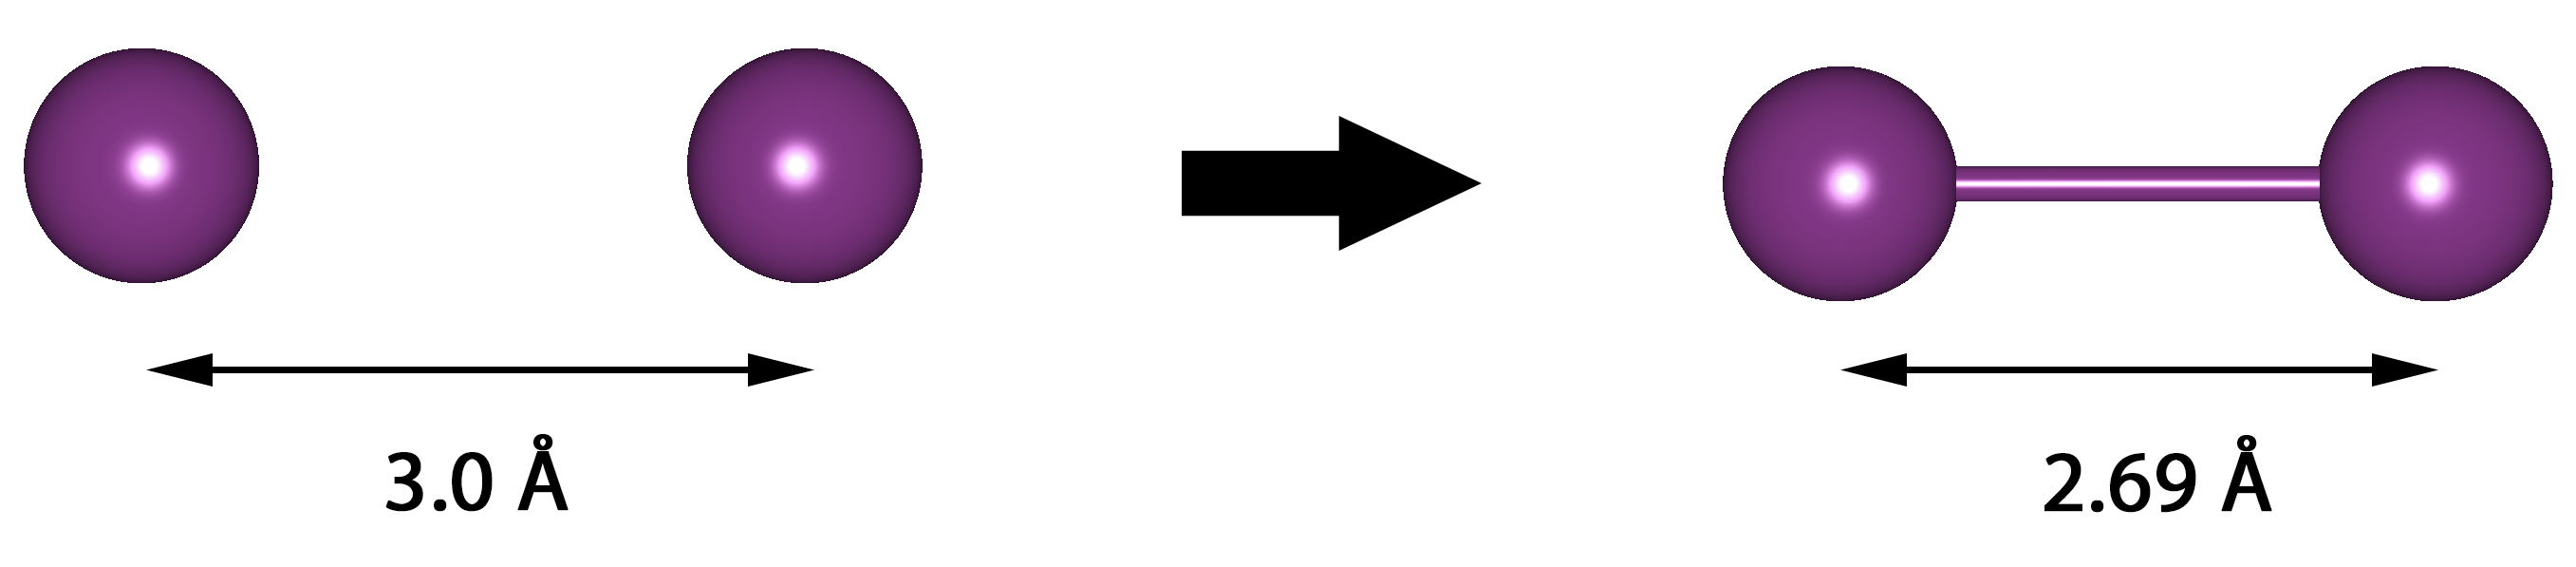
\includegraphics[width=14cm]{images/iodine_molecule.png}
\caption{Energy minimisation of two iodine atoms from an initial separation of 3.0 \r{A}.}
\label{figure:iodine_dimer}
\end{figure}

\subsection{+U study}
\label{subsection:plus_U}

In some DFT studies, an additional potential energy term (Hubbard U parameter or +U) is sometimes included to better capture the Coulomb interaction of localised electrons. An LDA or GGA functional alone will typically not describe this interaction correctly, especially for localised $d$ and $f$ electrons\footnote{Multiple occupation of $d$ and $f$ orbitals incurs an energy penalty which is not accurately modelled by the exchange-correlation functional.}. Of particular concern is the calculated value of the band gap from DFT simulations, as this value may deviate by up to 30\% from experimental values. Remedying this shortcoming with an appropriate +U parameter could therefore be valuable in obtaining accurate energies. 

In the literature, one GGA+U study of Fe-doped tetragonal \zirconia\ has shown that the inclusion of a +U term on Zr $d$ orbital electrons between 0 and 3.3 eV changes the electronic properties (in particular the electronic density of states) of the system significantly, and that the best agreement with experimental data occurs when U = 0 eV \cite{Sangalli2013}. Other GGA+U studies on bulk tetragonal \zirconia\ found that a +U term of 4 eV led to calculated lattice parameters which were in good agreement (within 0.05 \r{A}) with experimental values, but that the calculated band gap was still underestimated by 1.28 eV \cite{RuizPuigdollers2016, Chen2015, Puigdollers2015}. One LDA+U study in \zirconia\ used a +U parameter of 1 Ry (13.6 eV), and reproduced the correct order of stability of the monoclinic, tetragonal and cubic phase. This shows how the value of the +U parameter can vary significantly depending on the other approximations being used in the DFT calculations, and therefore an appropriate +U value for this thesis would have to be found independently. A +U study of the zirconium atom, with an electronic configuration of [Kr]$4d^{2}5s^{2}$, was performed to determine the response to and therefore the viability of this additional potential term for the $d$ electrons.

Figure \ref{Figure:plusubandgap} shows the effect on the calculated band gap when introducing a +U term. While the +U term does increase the band gap, the effect is not significant in bringing the prediction in-line with experimental values. Even with +U terms of 10 eV, the calculated band gap falls short of the experimental band gap by at least 1.5 eV. Moreover, with +U terms greater than 4 eV, we begin to see erratic behaviour in the development of both the band gap, and also in the predicted crystal structure. 

For the tetragonal phase, the calculated band gap (4.2 eV) does not agree with that calculated by Puigdollers \emph{et al.} (4.5 eV) when a +U term of 4 eV is used\cite{RuizPuigdollers2016}. The PBE GGA exchange-correlation functional and a plane-wave basis set was used in both studies, however, their study utilised the VASP 5.3 DFT software package while CASTEP 8.0 was used in this thesis. Different software packages may use different minimisation methods which could contribute to differing values, but determining the cause of this anomaly would require a separate study of the two codes at a low level which is beyond the scope of this thesis.

%Cubic is fine, it just keeps expanding with +U as we expect. The tetragonal phase expands in the short a&b directions but contracts in the long c direction (i.e. becomes more 'cubic') up until 6 eV, after which it grows in the same manner as cubic.

%The monoclinic phase is harder to explain. There is a cross-over in the length of the a and b parameter at around 4 eV, and then the beta angle (the ~99 deg between a and c) snaps into 90 deg at 11 eV, and when I look at the output structure at this energy, the coordination number of Zr is 6, down from 7. That's why the lattice parameters don't fall into a=b=c, because it doesn't become cubic.

%As you can see from the band gap plot below, just +U by itself is not enough to reproduce the experimental band gap, even for monoclinic. We're off by about 1.5 eV in each case.

\begin{figure}[ht] % +U band gaps
\begin{center}
\begin{tikzpicture}
	\begin{axis}
		[width=\linewidth*0.7, xlabel={+U on Zr \emph{d} orbitals (eV)}, ylabel={Band gap (eV)}, ymin=3.2, ymax=5, xmin=0, xmax=12, legend style={{draw=}, at={(0.35,0.95)}, anchor=north east, legend columns=1}]
		\addplot[no marks] table [x=plusU, y=bandgap,]{dat/plus_u_mono.dat}; \addlegendentry{Monoclinic};
        \addplot[no marks, dashed] table [x=plusU, y=bandgap, ]{dat/plus_u_tet.dat}; \addlegendentry{Tetragonal};
        \addplot[no marks, densely dotted, black] table [x=plusU, y=bandgap,]{dat/plus_u_cubic.dat}; \addlegendentry{Cubic};
			\end{axis}
		\end{tikzpicture}
		\caption{Calculated band gaps for different +U values in monoclinic, tetragonal and cubic \zirconia .}
		\label{Figure:plusubandgap}
	\end{center}
\end{figure}

\subsubsection{Monoclinic}

In monoclinic \zirconia , the use of a +U term causes the lattice parameters to change disproportionately to each other, as seen in Figure \ref{Figure:plusumono}. All lattice parameters increased with larger +U terms, however, expansion in the $a$ direction proceeded faster than in the $b$ direction, resulting in the $a$ lattice parameter becoming larger at a +U of 4 eV. +U terms larger than 10.5 eV caused the lattice parameters to snap suddenly onto new values. A  investigation of the atomic positions revealed that the monoclinic crystal structure had collapsed into an orthorhombic structure (i.e. the cell experienced a shear strain which resulted in a $\beta$ of 90\textdegree), with the co-ordination number of zirconium ions falling to 6 from 7.

\begin{figure}[ht] % +U mono
\begin{center}
\begin{tikzpicture}
	\begin{axis}
		[width=\linewidth*0.7, xlabel={+U on Zr \emph{d} orbitals (eV)}, ylabel={Lattice parameter (\r{A})}, ymin=4.9, ymax=6.3, xmin=0, xmax=12, legend style={{draw=}, at={(0.18,0.95)}, anchor=north east, legend columns=1}]
		\addplot[no marks] table [x=plusU, y=a,]{dat/plus_u_mono.dat}; \addlegendentry{$a$};
        \addplot[no marks, dashed] table [x=plusU, y=b, ]{dat/plus_u_mono.dat}; \addlegendentry{$b$};
        \addplot[no marks, densely dotted, black] table [x=plusU, y=c,]{dat/plus_u_mono.dat}; \addlegendentry{$c$};
			\end{axis}
		\end{tikzpicture}
		\caption{Individual lattice parameters as a function of +U term in monoclinic \zirconia .}
		\label{Figure:plusumono}
	\end{center}
\end{figure}

\subsubsection{Tetragonal}

In tetragonal \zirconia , increasing the +U term (Figure \ref{Figure:plusutet}) has a strong anisotropic effect on the lattice parameters. Unusually, the $c$ parameter falls (up to an +U energy of 6 eV) while the $a$ parameter increases. Typically it would be expected that both parameters would increase, perhaps at different rates, because the +U term increases the total energy (by increasing the Coulombic contribution) in the system. This increase in energy leads to higher stresses and therefore larger interatomic spacings (cells are permitted to relax in these calculations).

Systems will always tend towards the lowest energy configuration. Therefore the reduction of the $c$ parameter suggests that it is already in a high energy configuration in the $c$ direction (overextended) and can reduce its energy by being compressed in that direction (i.e. becoming more cubic). This is consistent with the interpretation that lower temperature phases of \zirconia\ are distortions of the cubic fluorite phase caused by a small cation radius. 

Above a +U parameter of 6 eV however, the $c$ parameter suddenly begins to increase. Upon further inspection of the resulting cell, it was found that it had transitioned completely to cubic fluorite from tetragonal. This can also be confirmed by observing that the relationship between the parameters becomes $2a^2 = c^2$ (i.e. the $c$ parameter is the same length as the unit cell's [110] diagonal, see Figure \ref{figure:tetvscubic}).

\begin{figure}[ht] % +U tet
\begin{center}
\begin{tikzpicture}
	\begin{axis}
		[width=\linewidth*0.7, xlabel={+U on Zr \emph{d} orbitals (eV)}, ylabel={$a$ parameter (\r{A})}, ymin=3.6, ymax=3.8, xmin=0, xmax=12, legend style={{draw=}, at={(0.18,0.95)}, anchor=north east, legend columns=1}, tick pos=left]
		\addplot[no marks] table [x=plusU, y=a,]{dat/plus_u_tet.dat}; \addlegendentry{$a$};
        %\addplot[no marks, dashed] table [x=plusU, y=b, ]{dat/plus_u_tet.dat}; \addlegendentry{b};
        \addplot[no marks, dashed, black] table [x=plusU, y=c,]{dat/plus_u_tet.dat}; \addlegendentry{$c$};
			\end{axis}
            \begin{axis}[width=\linewidth*0.7,
     xmin = 0, xmax = 12,
     ymin = 5.16, ymax = 5.32,
     hide x axis,
     hide y axis, tick pos=right]
     \addplot[no marks, dashed, black] table [x=plusU, y=c,]{dat/plus_u_tet.dat};
   			\end{axis}
            \pgfplotsset{every axis y label/.append style={rotate=180}}
   \begin{axis}[width=\linewidth*0.7,
         xmin=0, xmax=12,
         ymin=5.16, ymax=5.32,
         hide x axis,
         axis y line*=right,
         ylabel={$c$ parameter (\r{A})}
     ]
   \end{axis}
		\end{tikzpicture}
		\caption{Individual lattice parameters as a function of +U term in tetragonal \zirconia .}
		\label{Figure:plusutet}
	\end{center}
\end{figure}

\subsubsection{Cubic}

The effect of a +U term on a lattice parameter of cubic \zirconia\ is shown in Figure \ref{Figure:plusucubic}. Notably, the symmetry of the cell remains intact even up to a +U term of 12 eV, unlike in the monoclinic and tetragonal phases. The lattice parameter also increases superlinearly as the +U term is increased. This is the typical response that is expected when a +U term is introduced. 

\begin{figure}[ht] % +U cubic
\begin{center}
\begin{tikzpicture}
	\begin{axis}
		[width=\linewidth*0.7, xlabel={+U on Zr \emph{d} orbitals (eV)}, ylabel={Lattice parameter (\r{A})}, ymin=5.1, ymax=5.35, xmin=0, xmax=12, legend style={{draw=}, at={(0.18,0.95)}, anchor=north east, legend columns=1}]
		\addplot[no marks] table [x=plusU, y=a,]{dat/plus_u_cubic.dat}; \addlegendentry{$a$};
        %\addplot[no marks, dashed] table [x=plusU, y=b, ]{dat/plus_u_cubic.dat}; \addlegendentry{b};
        %\addplot[no marks, densely dotted, black] table [x=plusU, y=c,]{dat/plus_u_cubic.dat}; \addlegendentry{c};
			\end{axis}
		\end{tikzpicture}
		\caption{Lattice parameter as a function of +U term in cubic \zirconia .}
		\label{Figure:plusucubic}
	\end{center}
\end{figure}

There was however one instance of unexpected behaviour. Knowing that the tetragonal phase collapses to cubic at +U terms greater than 6 eV, we would expect both to exhibit the same band gap in this region. Looking at the band gap results from Figure \ref{Figure:plusubandgap}, we see that the band gaps of tetragonal and cubic \zirconia\ continue to be different above 6 eV, despite the crystal structures being the same in this region. One difference between the cells is that the cubic unit cell has 12 atoms while the tetragonal unit cell has 6 atoms. While this suggests a size effect, the band gap difference did not appear when comparing the band gaps of unit cells and supercells in the absence of a +U term. 

After considering the impact of a +U term in DFT calculations, the decision was made not to include the term. While it would provide a small improvement in the calculated band gap for the cubic phase, the effect on cell symmetry of the other phases would present a confounding variable, especially when placing defects into the structure. It is therefore more useful to run calculations without a +U term to maintain consistency of results between different phases in this thesis.